\chapter{Machine learning modeling}
Now that we have prepared our dataset in the form that could be used by any machine learning algorith, in this chapter we will train a number of classification machine learning alogorithms with grid search parameter optimization and cross validation for evaluation during the training stage. Best perfoming model selected based an appropriate model metric will be tested with the test set of our data set which was held back during model training. 

\textbf{Classification models}

The following list maching learning classification models will be tested.
\begin{itemize}
\item Logistic regression
\item Decision tree
\item Random Forest
\item Extreme Gradient boosting
\item K-Nearest Neighbourhood classifier
\end{itemize}

\section{K-fold training data split and cross-validation}
For each of the models listed above we use cross-validation to compare the performance of each model during the training. 
Cross validation is an essential technique when using the training data. It opens up a better of use the training data set through multiple model evaluation (K-fold) during the training phase. Briefly, it involves K-fold splitting of the training dataset where the training dataset is randomly split into K-folds or groups. During the training the first fold is kept for testing while the remaining K-1 group are used for training. The training is repeated k times and each time a different split group is used for validation. However, it is worth noting that each fold should be a good representative of the whole training dataset. Stratified K-fold attempts to solve this issue by preserving class ratio when fold groups are created. 

\section{The imbalanced dataset problem}
Clearly our data set is imbalanced and we have to re-sample it before model training. The impacts of imbalanced data are implicit, i.e. it does not raise an immediate error when you build and run your model, but the results can be delusive.
\subsection{How to deal with the imbalanced data}
Several solutions have been suggested in the literature to address this problem, amongst which are:

- \textbf{`Data-level techniques`} — At the data level, solutions work by applying re-sampling techniques to balance the dataset. These can be done by oversampling the minority class, which is to synthetically create new instances from existing ones; or under-sampling the majority class, which eliminates some instances in the majority class. However, both techniques can have their drawbacks. Oversampling new data can cause the classifier to over-fit; whereas under-sampling can discard essential information. A combination of both techniques with a heuristic approach can be found in specialized literature with excellent results.

- \textbf{`Algorithmic-level techniques`} —Algorithmic level solutions can be done by adjusting weighted costs accordingly to the number of training instances in each class. In parametric classifier like Support Vector Machine, grid search and cross-validation can be applied to optimise the $C$ and $\gamma$ values. For non-parametric classifier like the decision tree, adjusting the probabilistic estimate at the tree leaf can improve the performance.

- \textbf{`A combination of both`} — A hybrid approach is also constantly being explored in various literature, including AdaOUBoost (adaptive over-sampling and undersampling boost) proposed by Peng and Yao and Learning By Recognition, using the concept of auto association-based classification approach proposed by Japkowicz.

\subsubsection{Dealing with imbalanced data in Python}
One of the most popular libraries for sampling methods in Python is none other than the imbalanced-learn package. It provides several methods for both over- and under-sampling, as well as some combinations methods. 

- \textbf{Random under-sampling} with \hl{`RandomUnderSampler`}

- \textbf{`Oversampling`} with \hl{`SMOTE`} (Synthetic Minority Over-sampling Technique)

- \textbf{`Combination':}a combination of both random under-sampling and oversampling using pipeline

Reference for this notes are from a write up by Jack tan. The link is here \url{https://towardsdatascience.com/how-to-deal-with-imbalanced-data-in-python-f9b71aba53eb}

We balanced our dataset using SMOTE. Figure \ref{fig:smote_balanced} shows a histogram plot for the two classes (subscribed and not subscribed). It is clear that using SMOTE resulted to a well balanced dataset with 50:50 class ratio. 

\begin{figure}[tbh]
\centering
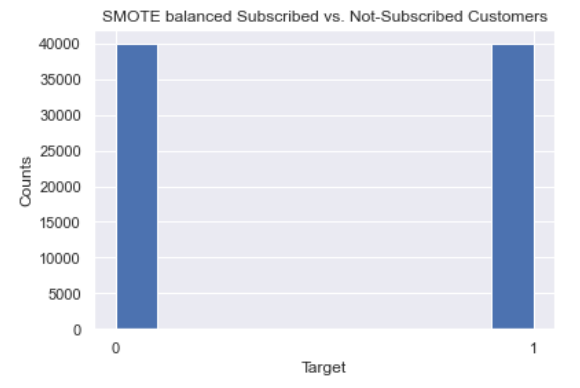
\includegraphics[width = 1.0\hsize]{./resources/img/fig_smote_balanced_count.png}
\caption{Table of evaluation metric values for 5 machine learning models.} 
\label{fig:smote_balanced}
\end{figure}

\section{Evaluation metric selection}
There are a number metrics that are routinely used to evaluate machine learning models. The metrics include:

- \textbf{\hl{Accuracy}} — the number of correct predictions made as a ratio of all predictions made.

- \textbf{\hl{ROC}} — calculated by plotting the true positive rate (TPR) against the false positive rate (FPR) at various threshold settings. The area under the curve is the ROC_Score.

- \textbf{\hl{Recall}} — quantifies the number of true positives found

- \textbf{\hl{Precision}} — quantifies the number of positive class predictions that actually belong to the positive class.

Since our dataset is imbalanced, using accuracy as metric would not be appropriate as any dummy could produce with a decent accuracy. I choose ROC_AUC as my metric of choice because of the imbalanced dataset with small positive class percentage. 

ROC analysis does not have any bias toward models that perform well on the majority class at the expense of the minority class — a property that is quite attractive when dealing with imbalanced data.
ROC is able to achieve this by looking into both the True positive rate (TPR) and False positive rate (FPR). We will get a high ROC if both the TPR and FPR are above the random line.


\section{Model evaluation}
After splitting our training dataset into 80:20 ratio using regular K-fold splitting and stratified K-fold splitting, we trained and evaluated each of the five classification machine learning algorithms listed above. Figure \ref{fig:kfold_metric} shows a table of the results of the metrics obtained using the two methods of k-fold splitting. We also have trained our model using the smote balanced dataset and the results are also incorporated in the figure. 
We see that using either stratified K-fold or balancing our dataset using smote resulted to marginal improvement in the value of \hl{AUC} score. The improvement is only for the case of K-Neighbourhood (KNN) classifier (an improvement from 0.62 to 0.63). For all the other models, when judged based on the AUC score, there is no real improvement in using stratfied k-fold or smote balancing our dataset.  

\begin{figure}[tbh]
\centering
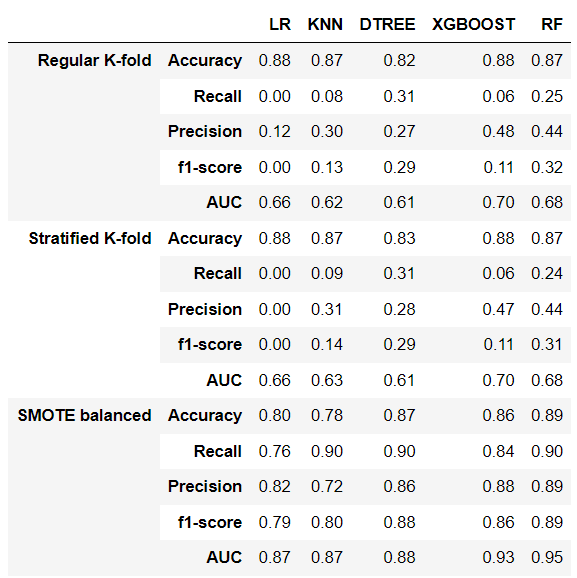
\includegraphics[width = 1.0\hsize]{./resources/img/fig_eval_metrics_kfold_and_smote.png}
\caption{Table of evaluation metric values for 5 machine learning models.} 
\label{fig:kfold_metric}
\end{figure}

Figure \ref{fig:auc_vs_accuracy} shows a scatter plot of \hl{AUC} versus \hl{Accuracy} for the five models. As can be seen \hl{XGBOOST} resulted with the highest AUC score (70\%) while still maintaining a high accuracy of 88\%. We therefore, choose XGBOOST as our base model. 

\begin{figure}[tbh]
\centering
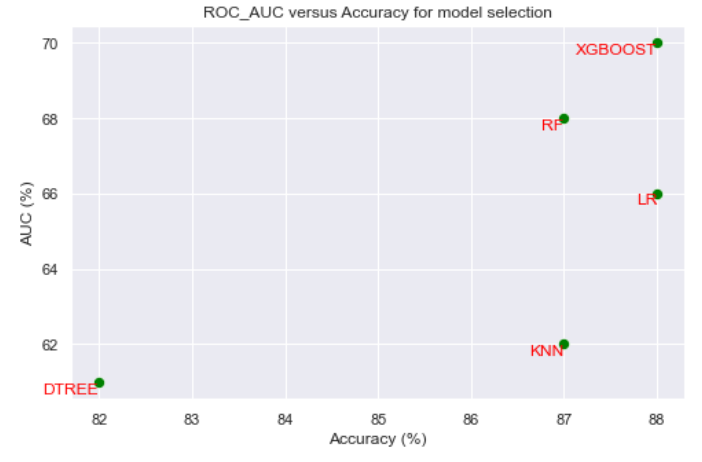
\includegraphics[width = 1.0\hsize]{./resources/img/fig_auc_vs_accuracy.png}
\caption{AUC score versus Accuracy showing XGBOOST performing the best.} 
\label{fig:auc_vs_accuracy}
\end{figure}
